% 编译顺序: xelatex -> bibtex -> xelatex -> xelatex
\documentclass[UTF8,AutoFakeBold=1,AutoFakeSlant,zihao=-4]{SCNU}

% ---------- 常用宏包 ----------
\usepackage{hyperref}
\usepackage{float}
\usepackage{enumitem}
\usepackage{graphicx}
\usepackage{amsmath}

% ---------- 基本信息（填写自己的） ----------
\newcommand{\thesisTitleEN}{Your English Title}

\newcommand{\yourTitle}{你的论文题目}
\newcommand{\yourTeacher}{指导教师}
\newcommand{\yourName}{你的姓名}
\newcommand{\studentID}{你的学号}
\newcommand{\yourDept}{学院}
\newcommand{\yourMajor}{专业}
\newcommand{\writingTime}{202X年X月}

% ---------- 正文开始 ----------
\begin{document}
	
	% 封面（自动生成）
	\coverpage
	
	% ================= 中文摘要 =================
	\begin{abstract}
		这里填写中文摘要内容。
		
		要求：
		1. 简要介绍研究背景
		2. 描述提出的方法
		3. 给出实验结果
		4. 总结贡献
		\keywords{关键词1，关键词2，关键词3}
	\end{abstract}
	
	% ================= 英文摘要 =================
	\begin{abstractEN}
		Write your English abstract here.
		\keywordsEN{keyword1, keyword2, keyword3}
	\end{abstractEN}
	
	% 目录
	\contentpage
	
	% ================= 正文 =================
	
	\section{绪论}
	
	\subsection{研究背景与意义}
	这里写研究背景。
	参考文献示例\cite{rottensteiner2014isprs}
	
	\subsection{国内外研究现状}
	这里写相关工作。
	
	\subsection{本文主要工作}
	\begin{enumerate}
		\item 工作1
		\item 工作2
		\item 工作3
	\end{enumerate}
	
	\subsection{本章小结}
	总结本章内容。
	
	% ================= 示例：公式 =================
	\section{相关理论基础}
	
	示例公式：
	\begin{equation}
		E = mc^2
	\end{equation}
	
	% ================= 示例：图片 =================
	\section{方法设计}
	
\begin{figure}[ht]
	\centering
	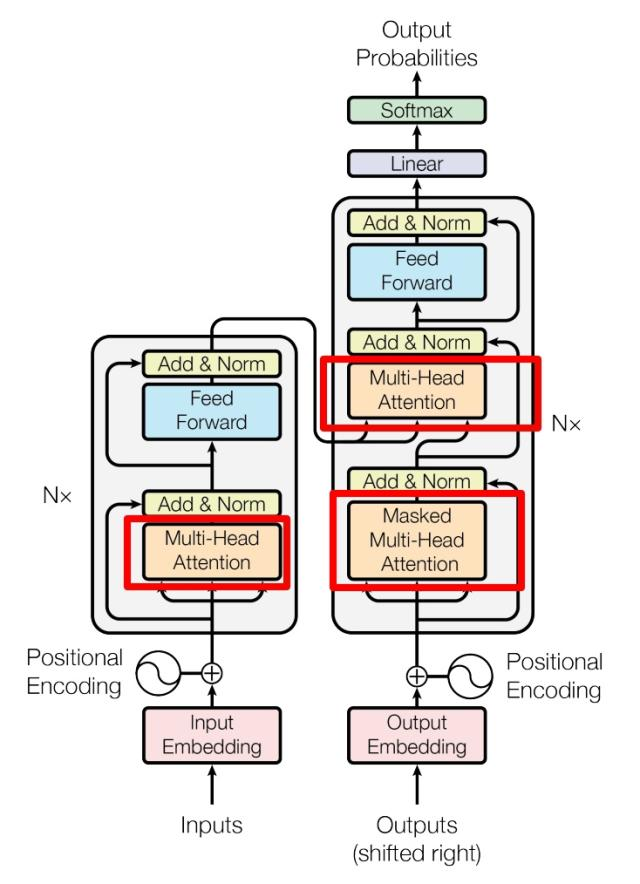
\includegraphics[width=0.5\textwidth]{imgs/workflow.png}
	\caption{示例图片}    \label{fig:workflow}
\end{figure}
	
	% ================= 示例：表格 =================
	\section{实验部分}
	
	\begin{table}[H]
		\centering
		\begin{tabular}{c|c}
			方法 & 精度 \\
			\hline
			方法A & 90\% \\
			方法B & 92\%
		\end{tabular}
		\caption{示例表格}
	\end{table}
	
	% ================= 结论 =================
	\section{总结与展望}
	
	总结本文工作，并提出未来研究方向。
	
% 参考文献（自动生成）
\begin{references}
	\bibliography{references.bib}
\end{references}
%\nonumsection{附录}


%\appendixformat    % 作为附录时，使用该命令为图表更新格式
\begin{acknowledgement}
	待写致谢。
\end{acknowledgement}
\end{document}